\documentclass[12pt,a4paper,twoside]{article}


%-------------------------------- My STY------------------------------------------------------------------

\usepackage[latin1]{inputenc}
\usepackage{amsmath, amsthm, amssymb, amsfonts,amscd, verbatim, mathrsfs}
\usepackage{setspace}
\usepackage{graphicx}
\usepackage[english]{babel}
\usepackage[a4paper]{geometry}
\usepackage{hyperref}
\usepackage{enumerate}
\usepackage{color}
\usepackage{rotating}
\usepackage{enumerate}
\usepackage{graphicx}
% \usepackage{mathtools}

\geometry{top=1.3in, bottom=1.4in, left=3.55cm, right=3.55cm}
\setlength{\parskip}{0.1cm}
\setlength{\parindent}{0cm}
  %------------------------------ My Environments -------------------------------------


\newtheoremstyle{upright}%
        {12pt plus2pt minus4pt}%
        {14pt plus2pt minus4pt}%
        {\upshape}%
        {}%
        {\bfseries\scshape\large}%
        {}%
        {1em}%
                      %
        {}%

\theoremstyle{upright}
\newtheorem{theorem}{Theorem}[section]
\newtheorem{lemma}[theorem]{Lemma}
\newtheorem{prop}[theorem]{Proposition}
\newtheorem{corollary}[theorem]{Corollary}
\newtheorem{axiom}[theorem]{Axiom}
\newtheorem{dfn}[theorem]{Definition}
\newtheorem{eg}[theorem]{Example}
\newtheorem{cor}[theorem]{Corollary}
\newtheorem{re}[theorem]{}


\newenvironment{prf}%
{\noindent \ignorespaces \large\textbf{Proof}\normalsize}%
{\qed}
%\begin{flushright}
%    $\blacksquare$
%\end{flushright} \par\noindent%
%\ignorespacesafterend

\newenvironment{fr}%
{\noindent \ignorespaces  \large\textbf{References and Further Reading}\normalsize}%



%-----------------------------------My commands-------------------------------------------------------------------------
\newcommand{\indentitem}{\setlength\itemindent{25pt}}
\newcommand{\smallindent}{\hspace{20pt}}
\newcommand{\midindent}{\hspace{52pt}}
\newcommand{\bfit}[1]{\textit{\textbf{#1}}}
\newcommand{\num}{\tag{\addtocounter{equation}{1}\arabic{equation}}}
\newcommand{\blankpage}{\mbox{} \newpage }
\DeclareMathOperator*{\argmax}{arg\,max}

\author{Patrick Robotham}
\title{AIXI Notes}
\begin{document}
\maketitle

This is a collection notes on the paper \cite{MC-AIXI} the emphasis is on description, most of the maths 
is glossed over.


\section{The set up}

We must attempt to solve the general reinforcement learning problem. 
An agent lives in some unknown environment, and interacts with the environment in cycles.
In each cycle, the agent must choose some action, and then the environment gives the agent 
an observation and a reward. The agent's job is to get as much reward as it can from this environment.

\subsection{String Notation}
A string $x_1 x_2 \ldots x_n$ of length $n$ is denoted $x_{1:n}$.

The prefix $x_{1:j}$ of $x_{1:n}$ where $j \leq n$ is denoted by $x_{\leq j}$ or $x_{< j+1}$.

$ax_{1:n}$ denotes $a_1 x_1 a_2 x_2 \ldots a_n x_n$.

$ax_<j$ denotes $a_1 x_1 a_2 x_2 \ldots a_{j-1} x_{j-1}$.

The empty string is denoted by $\epsilon$.

The concatenation of two strings $s$ and $r$ is denoted by $sr$.

\subsection{Formalizing the reinforcement learning problem}

$\mathscr{A}$ denotes the set of possible actions. 

$\mathscr{O}$ denotes the set of possible observations.

$\mathscr{R}$ denotes the set of possible rewards. 

$\mathscr{X}$ is the perception space $\mathscr{O} \times
\mathscr{R}$.

\dfn A history $h$ is an element of $(\mathscr{A} \times \mathscr{X})^* \cup 
(\mathscr{A} \times \mathscr{X})^* \times \mathscr{A}$.

\dfn An environment $\rho$ is a sequence of conditional probability functions
$\{\rho_0, \rho_1, \rho_2, \ldots \}$,
where $\rho_n : \mathscr{A}^n \to \text{Density}(\mathscr{X}^n)$, that satisfies
\[\forall a_{1:n} \forall x_{<n} : \rho_{n-1}(x_{<n} | a_{<n}) = 
\sum_{x_n \in \mathscr{X}} \rho_n(x_{1:n} | a_{1:n}).\]

This condition corresponds to actions have no effects on earlier perceptions.

Given an environment $\rho$, the predictive probability $p$ is defined as
\begin{equation}
p(x_n | ax_{<n}a_n) = \frac{\rho_n(x_{1:n} | a_{1:n})}{\rho_{n-1}(x_{<n} | a_{<n})}
\end{equation}

Thus 
\begin{equation}
\rho_n(x_{1:n} | a_{1:n}) = p(x_1 | a_1) p(x_2 | ax_1a_2) \cdots p(x_n |ax_{<n}a_n)
\end{equation}



\section{Planning}


MC-AIXI uses a technique called Monte-Carlo Tree Search to plan.

In our search tree, the nodes are histories. There are two types of nodes,
\emph{decision nodes} which end in observation-reward pairs, and \emph{chance nodes} which end in actions.

To each node $h$, we associate an estimate of its future reward $\hat V(h)$ and a visit count $T(h)$. 
The visit count is the number of times h has been sampled.


Monte-Carlo tree search has four phases that are endlessly cycled see 

\begin{enumerate}

\item Selection Phase: Traverse the search tree from the root to an existing leaf chance node $n$.
\item Expansion Phase: Add a new decision node as a child to $n$
\item Simulation Phase: Rollout $n$ with the environment $\rho$ to sample a possible future path
\item Backpropagation Phase: Update the value estimate for each node going from the end of the future path 
 back to the root.

\end{enumerate}


\begin{figure}
\centering
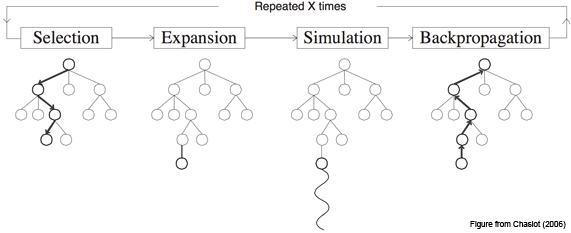
\includegraphics[scale=0.5]{mcts.png}
\caption{Sourced from http://www.cameronius.com/research/mcts/about/mcts-algorithm-1a.png}
\label{mcts}
\end{figure}


\blankpage


\subsection{Initialization}
We start with a search tree rooted at a single decision node containing $|\mathscr{A}|$ children,
one for each possible action.
\subsection{Selection / Expansion}

Selection and expansion are combined in to a single step, since the selection is such that a non-leaf node may select as its child a node with visit count 0.

MC-AIXI traverses the search tree as follows.
Assume rewards are bounded in the interval $[\alpha, \beta]$ and that $m$ is the search horizon. 

If the current node $h$ is a decision node, the action picked is:
\begin{equation}
a_{Sel}(h) = \argmax_{a \in \mathscr{A}} 
\begin{cases} \frac{1}{m(\beta-\alpha)} \hat V (ha) + C \sqrt{\frac{log(T(h))}{T(ha)}}& \mbox{if } T(ha) > 0
\\ \infty & otherwise
 \end{cases}
\end{equation}

If there are multiple maximal actions, one is chosen at random.
(I stole this hueristic from the MC-AIXI paper, I don't understand it)
If the current node $ha$ is a chance node, the observation-reward pair $or$ 
is randomly picked according to the probability distribution given by $p(.|ha)$.

\subsection{Expansion}
Since the selection algorithm is such that a non-leaf node may select as its child node a node which has yet to 
be generated, the line between selection and expansion is blurry. We say a node is expanded if the node it picks
has a visit count of zero.
\subsection{Simulation}
We now get to the Monte-Carlo bit of Monte Carlo Search Trees: Simulation.

The simulation is done as follows. We rollout until we reach the search horizon $m$ to estimate the sum of 
future rewards. This rollout is done like so:

 We have a rollout policy $\Pi$ that picks an action at a decision node. $\Pi$ by default selects actions randomly.
Observation-reward pairs from chance nodes during rollout are generated as usual.   
\subsection{Backpropagation}

After rollout, we have a path of nodes $n_1n_2 \ldots n_m$.
Let $n_k$ be the the first unvisited node in this path. 

Let $r_j$ be the reward of the node $n_j$. $r_j = 0$ if $n_j$ is a chance node.

Then for each $j$ from $1$ to $k$, the estimated reward of $n_j$ is updated as follows:

\begin{equation}
\hat V (n_j) \leftarrow \frac{T(n_j)}{T(n_j) + 1} \hat V(n_j) + \frac{1}{T(n_j)+1} \sum_{i=j}^{m}r_i
\end{equation}

Furthermore, the visit count of each node $n_1 n_2 \ldots n_k$ is increased by 1.
\section{Predicting}

Our model class is all d-order Markov models. Markov models are represented using prediction suffix trees.


\subsection{The KT Estimator}
Let $Y$ be a bitstring.
Then 
\[
Pr_{KT}(Y_{n+1} \mid Y_{1:n}) =
\frac{\text{\# of 1s in $Y_{1:n}$} + 1/2}{n+1}
\]

$Pr_{KT}$ only depends on the number of 0s and 1s of $Y$. Thus, $Pr_{KT}$ is 
invariant under permutations.

\theorem
\begin{equation}
Pr_{KT}(0^a 1^b) = \frac{\displaystyle \prod_{i=0}^{a-1}{(1/2 + i)} \prod_{i=0}^{b-1}{(1/2 + i)}}
{\displaystyle(a+b)!}
\end{equation}

\subsection{Prediction Suffix Trees}

\dfn
A \emph{prediction suffix tree} $(M,\theta)$ is a proper binary tree where each leaf node
$l$ is equipped with a probability distribution $\theta(l)$
over $\{0,1\}$.

{\bf\underline {Notation:}}
Let $M$ be a binary tree. Let $s$ be a bitstring.
$M_s$ is the node in $M$ reached by the following algorithm:

\begin{verbatim}
set M_s = M.root

for c in s:
    If M_s is a leaf node:
        return M_s
    If c == 0
        M_s = M_s.right
    If c == 1
        M_s = M_s.left
endfor
return M_s

\end{verbatim}

\subsection{Calculating Probabilities With Prediction Suffix Trees}
Let $(M, \theta)$ be a prediction suffix tree.
Let $d$ be the depth of $M$.
Let $s$ be a bitstring. Assume $|s| > d$. Let $n$ satisfy $d < n < s$.


Then $Pr_M(s_{n+1} | s_{1:n})$ is calculated as follows:

\begin{enumerate}
\item Let $s' = \text{reverse}(s_{1:n})$.
\item Return $\theta(M_{s'})$.
\end{enumerate}

\subsection{Coding Proper Binary Trees}

We assume we have an upper bound $D$ for the proper binary tree $M$. We then code the tree by calling the function below with $M\text{.root}$.
(The idea of this code is that we preform a pre-order traversal, writing down 1 for internal nodses, 0 for leaf nodes of length less than D, and nothing otherwise.)

\begin{verbatim}

function code(node,depth){
 if(node.leaf() == true){
   if(depth < D){
      message += 0;
   }
 } else {
   message += 1;    
   code(node.left, depth+1);
   code(node.right, depth+1);
 }
}
message = [];
code(M.root, 0);
\end{verbatim}

We denote the length of this code by $\Gamma_D(M)$.

\subsection{Context Trees}

Context Trees are a way of working with a mixture of all Prediction Suffix Trees of depth at most $D$.


\dfn

A context tree of depth $D$ is a complete binary tree of depth $D$ where every 
node $n$ (including non-leaf nodes) is equipped with a bitstring, denoted $n\text{.bitstring}$.


\subsection{Updating Context Trees}

We initially start with a context tree where each node is equipped with just the empty string.
We set aside the first $D$ bits gained from interacting with the environment to a variable $h$.

Then, given a new bit $b$, we update the bitstrings in the context tree $M$ as follows:
(Note that we only update the context trees using bits from observation-reward pairs).

\begin{verbatim}
node = M.root;
context = reverse(h);
i = 1;
while(node is not a leaf){
  node.bitstring += b;
  if(context[i] = 1){
    node = node.left
    i += 1;
  } else {
    node = node.right
    i += 1;
  }
}
h = h+b;
\end{verbatim}
 

\subsection{Calculating Probabilities using Context Trees}

The function used to calculate the probability of the next bit of the sequence being 1 is given below.
Here $\texttt{prkt}$ is the KT estimator $Pr_{KT}$. Note that since we only use the KT estimator, it is
not necessary to keep track of the whole bitstring. We just need to keep track of the number of 1s and 0s.

\begin{verbatim}
function wprob(node){
  if(node.leaf == true){
    return prkt(node.bitstring);
  } else {
    return 0.5*prkt(node.bitstring) + 0.5*wprob(node.left)*wprob(node.right);
  }
}

\end{verbatim}

$\texttt{wprob}(M.root)$ gives a solomonoff-like probability estimate that the next bit in the sequence will be 1.

The equation is that after seeing $h = ax_{1:t-1}$, and deciding an action $a_t$,

\begin{equation}
\texttt{wprob}(root) = \sum_{M \in C_D}2^{-\Gamma_D(M)} Pr_M(x_t \mid  ax_{1:t-1}a_t)
\end{equation}

where $C_D$ is the set of all proper binary trees (which are turned in to prediction suffix trees
 by taking the KT estimator).

\subsection{The Factored Action-Conditional Context Tree Weighting Algorithm}

For this algorithm, we create $l_x$ different context trees in order to incorporate type information.

\begin{enumerate}
\item Initialize $ h = \epsilon , t = 1$. Create $l_x$ context trees.
\item While $|h| < D$, pick action $a_t$ randomly, observe $x_t$ set $h = hax, t = t+1$.
\item Determine action $a_t$, set h = $ha_t$.
\item Receive $x_t$. For each bit $x_t[i]$ of $x_t$, update the $i$th context tree with bit $x_t[i]$ using history
$hx[1,i-1]$ and recompute $wprob(root_i)$.
\item Set $x = hx_t, t = t+1$. Goto 3.
\end{enumerate}

\section{Pseudocode for MC-AIXI}

\begin{fr}
\bibliographystyle{unsrt}
\bibliography{thesis}

\end{fr}

\end{document}
